% Modern version of tac_rules.tex
% Compile with: latexmk -lualatex -shell-escape tac_rules_modern.tex
\documentclass[aspectratio=169,11pt,xcolor=table]{beamer}

%% ── Packages ──────────────────────────────────────────────────────────────
\usefonttheme{professionalfonts}
\usepackage{fontspec}
\usepackage{tikz}
\usetikzlibrary{arrows.meta, positioning, shapes.misc, calc}
\usepackage{minted}
\usepackage{mathpartir}
\usepackage{amsmath}
\usepackage{booktabs}
\usepackage[most]{tcolorbox}

%% ── Fonts ─────────────────────────────────────────────────────────────────
\setsansfont{Inter}[
  Extension      = .otf,
  UprightFont    = *-Regular,
  BoldFont       = *-SemiBold,
  ItalicFont     = *-Italic,
  BoldItalicFont = *-SemiBoldItalic]
\setmonofont{IBMPlexMono}[
  Extension      = .otf,
  UprightFont    = *-Regular,
  BoldFont       = *-SemiBold,
  ItalicFont     = *-Italic,
  Scale          = 0.92]
\newfontfamily\displayfont{Inter}[Extension=.otf, UprightFont=*-Bold]
\newfontfamily\lightfont{Inter}[Extension=.otf, UprightFont=*-Light]

%% ── Palette ───────────────────────────────────────────────────────────────
\definecolor{ink}{HTML}{0F172A}        % slate-900
\definecolor{bodytxt}{HTML}{1E293B}    % slate-800
\definecolor{muted}{HTML}{64748B}      % slate-500
\definecolor{hair}{HTML}{E2E8F0}       % slate-200
\definecolor{surface}{HTML}{F8FAFC}    % slate-50
\definecolor{accent}{HTML}{4F46E5}     % indigo-600
\definecolor{accentsoft}{HTML}{EEF2FF} % indigo-50
\definecolor{accentlite}{HTML}{A5B4FC} % indigo-300

%% Diagram colours (same names as the original deck)
\definecolor{clrArt}{HTML}{EEF2FF}     % artifact fill   (indigo-50)
\definecolor{clrArtBd}{HTML}{4F46E5}   % artifact border (indigo-600)
\definecolor{clrStg}{HTML}{FEF3C7}     % condition fill  (amber-100)
\definecolor{clrStgBd}{HTML}{D97706}   % condition border(amber-600)
\definecolor{clrT}{HTML}{059669}       % true exit       (emerald-600)
\definecolor{clrF}{HTML}{E11D48}       % false exit      (rose-600)

%% ── Beamer theme (self-contained) ─────────────────────────────────────────
\setbeamersize{text margin left=2.2em, text margin right=2.2em}
\setbeamertemplate{navigation symbols}{}

\setbeamercolor{normal text}{fg=bodytxt, bg=white}
\setbeamercolor{background canvas}{bg=white}
\setbeamercolor{structure}{fg=accent}
\setbeamercolor{frametitle}{fg=ink}
\setbeamercolor{alerted text}{fg=accent}
\setbeamercolor{item}{fg=accent}

\setbeamerfont{frametitle}{size=\Large, series=\bfseries}
\setbeamerfont{kicker}{size=\scriptsize, series=\bfseries}

\setbeamertemplate{itemize item}{%
  \raisebox{0.18em}{\tikz\fill[accent, rounded corners=0.6pt] (0,0) rectangle (0.32em,0.32em);}}
\setbeamertemplate{itemize subitem}{%
  \raisebox{0.2em}{\tikz\draw[accent, line width=0.6pt] (0,0) circle (0.13em);}}
\setbeamertemplate{enumerate item}{%
  \tikz[baseline=(n.base)]\node[circle, fill=accent, text=white, inner sep=0pt,
    minimum size=1.15em, font=\scriptsize\bfseries] (n) {\insertenumlabel};}

%% Kicker above each frame title: current part, or the deck name
\newcommand{\kickertext}{%
  \ifnum\value{section}>0 Part~\Roman{section}\enspace·\enspace\insertsectionhead
  \else MiniC\enspace·\enspace Code Generation\fi}

\setbeamertemplate{frametitle}{%
  \vskip1.0em
  {\usebeamerfont{kicker}\color{accent}\addfontfeature{LetterSpace=6}%
   \MakeUppercase{\kickertext}\par}%
  \vskip0.25em
  {\usebeamerfont{frametitle}\usebeamercolor[fg]{frametitle}%
   \displayfont\insertframetitle\par}%
  \vskip0.2em
}

\setbeamertemplate{footline}{%
  \begin{tikzpicture}
    \useasboundingbox (0,0) rectangle (\paperwidth,1.7em);
    \node[anchor=west, font=\tiny, text=muted] at (2.2em,0.95em)
      {MiniC\enspace·\enspace Three Address Code};
    \node[anchor=east, font=\tiny\bfseries, text=muted] at ($(\paperwidth,0.95em)+(-2.2em,0)$)
      {\insertframenumber\,/\,\inserttotalframenumber};
    \fill[hair] (0,0) rectangle (\paperwidth,0.22em);
    \fill[accent] (0,0) rectangle
      ({\paperwidth*\insertframenumber/\inserttotalframenumber},0.22em);
  \end{tikzpicture}}

%% Blocks as cards with an accent stripe
\setbeamertemplate{block begin}{%
  \par\vskip0.2em
  \begin{tcolorbox}[enhanced, breakable=false,
      colback=surface, colframe=hair, boxrule=0.5pt, arc=5pt,
      borderline west={2.5pt}{0pt}{accent},
      left=8pt, right=6pt, top=3pt, bottom=4pt,
      colbacktitle=surface, coltitle=accent,
      fonttitle=\scriptsize\bfseries, titlerule=0pt,
      toptitle=4pt, bottomtitle=0pt, lefttitle=8pt,
      title={\addfontfeature{LetterSpace=4}\MakeUppercase{\insertblocktitle}}]%
  \usebeamercolor[fg]{normal text}}
\setbeamertemplate{block end}{\end{tcolorbox}\vskip0.1em}

%% Title page: dark, full bleed
\setbeamertemplate{title page}{%
  \begin{tikzpicture}[remember picture, overlay]
    \fill[ink] (current page.south west) rectangle (current page.north east);
    % dot grid
    \foreach \x in {0,...,13} \foreach \y in {0,...,10}
      \fill[white, opacity=0.07]
        ($(current page.south east)+(-0.6cm-\x*0.42cm, 0.6cm+\y*0.42cm)$) circle (1.1pt);
    % ghost TAC snippet
    \node[anchor=south east, align=left, font=\ttfamily\large, text=accentlite,
          opacity=0.55] at ($(current page.south east)+(-1.4cm,1.3cm)$)
      {t1 := a + b\\t2 := t1 * c\\x\ \ := t2};
    % accent bar + text
    \fill[accent] ($(current page.north west)+(1.4cm,-2.2cm)$) rectangle ++(1.6cm,0.13cm);
    \node[anchor=north west, align=left, text width=11cm, inner sep=0pt]
      at ($(current page.north west)+(1.4cm,-2.75cm)$) {%
        {\color{accentlite}\scriptsize\bfseries\addfontfeature{LetterSpace=10}%
          MINIC\enspace·\enspace COMPILER CONSTRUCTION}\par\vskip0.6em
        {\color{white}\displayfont\fontsize{34}{38}\selectfont\inserttitle}\par\vskip0.5em
        {\color{white!75!ink}\lightfont\Large\insertsubtitle}\par\vskip1.4em
        {\color{white!55!ink}\small\insertdate}};
  \end{tikzpicture}}

%% Section divider: dark, big roman numeral
\setbeamertemplate{section page}{%
  \begin{tikzpicture}[remember picture, overlay]
    \fill[ink] (current page.south west) rectangle (current page.north east);
    \node[anchor=east, text=white, opacity=0.06, inner sep=0pt,
          font=\displayfont\fontsize{200}{200}\selectfont]
      at ($(current page.east)+(-1.2cm,0)$) {\Roman{section}};
    \fill[accent] ($(current page.west)+(1.4cm,-1.15cm)$) rectangle ++(1.6cm,0.13cm);
    \node[anchor=south west, align=left, text width=12cm, inner sep=0pt]
      at ($(current page.west)+(1.4cm,-0.5cm)$) {%
        {\color{accentlite}\small\bfseries\addfontfeature{LetterSpace=10}%
          PART \Roman{section}}\par\vskip0.4em
        {\color{white}\displayfont\fontsize{38}{42}\selectfont\insertsectionhead}};
  \end{tikzpicture}}
\AtBeginSection{\begin{frame}[plain,noframenumbering]\sectionpage\end{frame}}

%% ── Code ──────────────────────────────────────────────────────────────────
\setminted{style=xcode}

%% ── Control-flow diagram styles ───────────────────────────────────────────
%% cnd: a condition (jumping code with a T and an F exit)
%% blk: straight-line code (statement / basic block)
\tikzset{
  cfg/.style  = {font=\sffamily\scriptsize},
  cnd/.style  = {rectangle, rounded corners=4pt, draw=clrStgBd, fill=clrStg,
                 line width=0.7pt, minimum width=1.3cm, minimum height=0.55cm,
                 font=\ttfamily\scriptsize},
  blk/.style  = {rectangle, rounded corners=2pt, draw=clrArtBd, fill=clrArt,
                 line width=0.7pt, minimum width=1.3cm, minimum height=0.55cm,
                 font=\ttfamily\scriptsize},
  flow/.style = {-Stealth, line width=0.8pt, draw=muted},
  line/.style = {line width=0.8pt, draw=muted},
  tarr/.style = {-Stealth, line width=0.9pt, draw=clrT},
  farr/.style = {-Stealth, line width=0.9pt, draw=clrF},
  tf/.style   = {font=\sffamily\tiny\bfseries, inner sep=1pt},
  lbl/.style  = {font=\ttfamily\scriptsize, text=muted, inner sep=1pt},
  exit/.style = {font=\scriptsize, inner sep=1pt},
}

%% ── Notation shorthands ───────────────────────────────────────────────────
\newcommand{\trExpr}[1]{\mathit{trExpr}(#1)}
\newcommand{\trStmt}[1]{\mathit{trStmt}(#1)}
\newcommand{\trFun}[1]{\mathit{trFun}(#1)}
\newcommand{\trCond}[2]{\mathit{trCond}(#1,\;#2)}
\newcommand{\trJump}[3]{\mathit{trJump}(#1,\;#2,\;#3)}
\newcommand{\cat}{\mathbin{+\!\!+}}
\newcommand{\mln}[1]{\hbox{$\displaystyle\strut#1$}}
\newcommand{\tc}[1]{\texttt{#1}}

%% Rule names: Inter has no small caps, so use tracked uppercase in accent
\DeclareRobustCommand{\rulename}[1]{%
  {\bfseries\color{accent}\addfontfeature{LetterSpace=5}\MakeUppercase{#1}}}
\let\textsc\rulename
\renewcommand{\TirNameStyle}[1]{{\scriptsize\rulename{#1}}}

%% ── Meta ──────────────────────────────────────────────────────────────────
\title{Code Generation}
\subtitle{From Annotated AST to Three Address Code}
\author{}
\date{\today}

\begin{document}

\begin{frame}[plain,noframenumbering]\titlepage\end{frame}

%% ══════════════════════════════════════════════════════════════════════════
%% Compiler Pipeline
%% ══════════════════════════════════════════════════════════════════════════
\begin{frame}{Compiler Pipeline}
\centering
\resizebox{0.98\textwidth}{!}{%
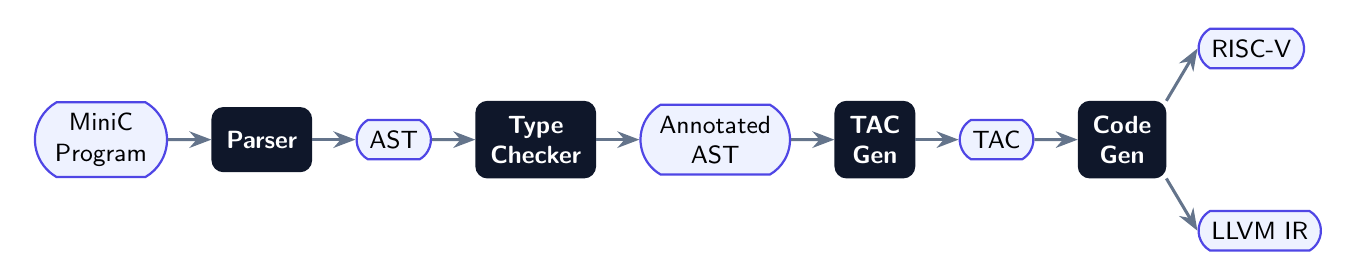
\begin{tikzpicture}[
  art/.style = {
    rounded rectangle,
    rounded rectangle arc length=120,
    draw=clrArtBd, fill=clrArt, line width=0.8pt,
    font=\sffamily\small, inner sep=4pt, align=center
  },
  stg/.style = {
    rectangle, rounded corners=4pt,
    draw=ink, fill=ink, text=white, line width=0.8pt,
    font=\sffamily\small\bfseries, inner sep=5pt, align=center,
    minimum height=0.8cm
  },
  arr/.style  = {-Stealth, line width=1.1pt, color=muted},
  node distance = 0.55cm
]
  \node[art]                            (minic)   {MiniC\\Program};
  \node[stg, right=of minic]            (parser)  {Parser};
  \node[art, right=of parser]           (ast)     {AST};
  \node[stg, right=of ast]              (tc)      {Type\\Checker};
  \node[art, right=of tc]               (aast)    {Annotated\\AST};
  \node[stg, right=of aast]             (tacgen)  {TAC\\Gen};
  \node[art, right=of tacgen]           (tac)     {TAC};
  \node[stg, right=of tac]              (codegen) {Code\\Gen};
  \node[art, above right=0.4cm and 0.55cm of codegen] (riscv) {RISC-V};
  \node[art, below right=0.4cm and 0.55cm of codegen] (llvm)  {LLVM IR};

  \draw[arr] (minic)              -- (parser);
  \draw[arr] (parser)             -- (ast);
  \draw[arr] (ast)                -- (tc);
  \draw[arr] (tc)                 -- (aast);
  \draw[arr] (aast)               -- (tacgen);
  \draw[arr] (tacgen)             -- (tac);
  \draw[arr] (tac)                -- (codegen);
  \draw[arr] (codegen.north east) -- (riscv.west);
  \draw[arr] (codegen.south east) -- (llvm.west);
\end{tikzpicture}%
}

\vspace{0.2em}
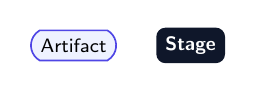
\begin{tikzpicture}[baseline, node distance=0.5cm]
  \node[rounded rectangle, rounded rectangle arc length=120,
        draw=clrArtBd, fill=clrArt, line width=0.6pt,
        font=\sffamily\scriptsize, inner sep=3pt] (a) {Artifact};
  \node[rectangle, rounded corners=3pt, draw=ink, fill=ink, text=white, line width=0.6pt,
        font=\sffamily\scriptsize\bfseries, inner sep=3pt, right=0.5cm of a] {Stage};
\end{tikzpicture}
\end{frame}

%% ══════════════════════════════════════════════════════════════════════════
%% What is Three Address Code?
%% ══════════════════════════════════════════════════════════════════════════
\begin{frame}{Three Address Code}
  \begin{block}{Definition}
    An intermediate representation in which each instruction involves
    \textbf{at most three addresses}: a result and up to two operands.
    Intermediate values are made explicit through fresh \emph{temporaries}.
  \end{block}
\end{frame}

\begin{frame}{Three Address Code: Instruction Forms}
  \smallskip
  \textbf{Instruction forms used in MiniC:}
  \begin{center}
    \scriptsize
    \rowcolors{2}{white}{surface}
    \begin{tabular}{lll}
      \toprule
      \textbf{Form}                  & \textbf{Syntax}                    & \textbf{Semantics}                 \\
      \midrule
      Copy assignment                & \tc{x := y}                        & $x \leftarrow y$                   \\
      Unary / binary assignment      & \tc{t := -a} \quad \tc{t := a + b} \quad \tc{t := a < b} & $t \leftarrow \ominus a$, $t \leftarrow a \oplus b$ \\
      Indexed load / store           & \tc{t := a[i]} \quad \tc{a[i] := y} & read / write memory at $a + i$   \\
      Cond.\ jump (relational)       & \tc{if a < b goto L}               & jump if $a < b$                    \\
      Cond.\ jump (boolean)          & \tc{if a goto L} \quad \tc{if\_false a goto L} & jump if $a$ is true / false \\
      Unconditional jump             & \tc{goto L}                        & always jump to $L$                 \\
      Label                          & \tc{L:}                            & marks a jump target                \\
      Procedure call                 & \tc{param a} \quad \tc{t := call f, n} & pass argument; call $f$ with $n$ args \\
      Return                         & \tc{return} \quad \tc{return a}    & leave the current function         \\
      \bottomrule
    \end{tabular}
  \end{center}

  \smallskip
  \textbf{Addresses} are one of: a variable name, a constant literal,
  or a fresh temporary (\tc{t1}, \tc{t2}, \ldots).
\end{frame}


%% ══════════════════════════════════════════════════════════════════════════

%% ══════════════════════════════════════════════════════════════════════════
\section{Intuition}
%% ══════════════════════════════════════════════════════════════════════════
%% ══════════════════════════════════════════════════════════════════════════

%% ── Expressions ──────────────────────────────────────────────────────────
\begin{frame}[fragile]{Expressions: Flattening the Tree}
  \begin{columns}[T]
    \begin{column}{0.44\textwidth}
      \begin{block}{Example}
        \begin{minted}[fontsize=\small]{c}
x = (a + b) * c; // 4 addresses!
        \end{minted}
        \vspace{0.3em} \pause
        \begin{minted}[fontsize=\small]{text}
t1 := a + b
t2 := t1 * c
x  := t2
        \end{minted}
      \end{block}
    \end{column} \pause
    \begin{column}{0.52\textwidth}
      \textbf{Idea.} An expression tree is \emph{flattened} bottom-up:
      \begin{itemize}
        \item Leaves (variables, constants) are already addresses — no code.
        \item Each inner node evaluates its children first (left to right),
              then stores its own result in a \textbf{fresh temporary}.
        \item The result of translating an expression is a pair:
              \emph{the code} and \emph{the address holding its value}.
      \end{itemize}
    \end{column}

  \end{columns}
\end{frame}

%% ── Booleans as values ──────────────────────────────────────────────────
\begin{frame}[fragile]{Boolean Operators: Short-Circuit}
  \begin{columns}[T]
    \begin{column}{0.44\textwidth}
      \textbf{Idea.} \tc{\&\&}, \tc{||} and \tc{!} produce a value like
      any other operator, but their code contains \emph{jumps}:
      \begin{enumerate}
        \item evaluate the left operand;
        \item if it already decides the result, skip the right operand;
        \item store \tc{true} or \tc{false} into a fresh temporary;
        \item both paths meet at an exit label.
      \end{enumerate}
      Short-circuit is preserved: \tc{b} is not evaluated when \tc{a} is false.
    \end{column}
    \begin{column}{0.27\textwidth}
      \begin{block}{\tc{x = a \&\& b;}}
        \begin{minted}[fontsize=\scriptsize]{text}
if_false a goto L1
if_false b goto L1
t1 := true
goto L2
L1:
t1 := false
L2:
x := t1
        \end{minted}
      \end{block}
    \end{column}
    \begin{column}{0.27\textwidth}
      \begin{block}{\tc{x = !flag;}}
        \begin{minted}[fontsize=\scriptsize]{text}
if_false flag goto L1
t1 := false
goto L2
L1:
t1 := true
L2:
x := t1
        \end{minted}
      \end{block}
    \end{column}
  \end{columns}
\end{frame}

%% ── Booleans as values: || and relational ───────────────────────────────
\begin{frame}[fragile]{Boolean Operators: \tc{||} and Relational Operators}
  \begin{columns}[T]
    \begin{column}{0.48\textwidth}
      \begin{block}{\tc{x = a || b;}}
        \begin{minted}[fontsize=\scriptsize]{text}
if_false a goto L2   ; a false: try b
goto L1              ; a true: skip b
L2:
if b goto L1
t1 := false
goto L3
L1:
t1 := true
L3:
x := t1
        \end{minted}
      \end{block}
      \scriptsize
      If \tc{a} is true we jump straight to \tc{L1} — \tc{b} is
      \textbf{not evaluated}. The pair \tc{if\_false a goto L2 / goto L1}
      is just \tc{if a goto L1} written the long way; a peephole pass
      simplifies it.
    \end{column}
    \begin{column}{0.48\textwidth}
      \begin{block}{\tc{b = x < y;}}
        \begin{minted}[fontsize=\scriptsize]{text}
t1 := x < y
b  := t1
        \end{minted}
      \end{block}
      \scriptsize
      Relational operators need \textbf{no jumps} when used as values:
      TAC has a binary assignment for them, like for \tc{+}.

      \medskip
      Conditions in \tc{if} and \tc{while} reuse exactly this code:
      compute the value, then test it (next slide).

      \medskip
      (A target without such an instruction would use the
      \tc{t := true / t := false} pattern instead.)
    \end{column}
  \end{columns}
\end{frame}

%% ── Conditions: value, then test ────────────────────────────────────────
\begin{frame}[fragile]{Conditions}
  \begin{columns}[T]
    \begin{column}{0.52\textwidth}
      \small
      A condition is just a boolean expression: compute its
      \textbf{value} with $\mathit{trExpr}$, then test it with a
      \textbf{single jump}.
      \begin{center}
        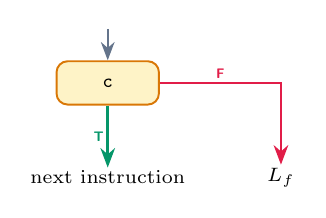
\begin{tikzpicture}[cfg]
          \node[cnd]  (c)  at (0,0)      {c};
          \node[exit] (nx) at (0,-1.2)   {next instruction};
          \node[exit] (lf) at (2.2,-1.2) {$L_f$};
          \draw[flow] ($(c.north)+(0,0.4)$) -- (c.north);
          \draw[tarr] (c.south) -- node[tf, left, text=clrT] {T} (nx.north);
          \draw[farr] (c.east) -| node[tf, pos=0.25, above, text=clrF] {F} (lf.north);
        \end{tikzpicture}
      \end{center}
      \begin{itemize}
        \item \textbf{F exit}: \tc{if\_false a goto Lf}.
        \item \textbf{T exit}: no jump at all; execution
              \emph{falls through}.
      \end{itemize}
      The enclosing statement only decides $L_f$.
    \end{column}
    \begin{column}{0.44\textwidth}
      \begin{block}{Relational: \tc{x < y}}
        \begin{minted}[fontsize=\footnotesize]{text}
t1 := x < y
if_false t1 goto Lf
        \end{minted}
      \end{block}
      \begin{block}{Boolean variable: \tc{flag}}
        \begin{minted}[fontsize=\footnotesize]{text}
if_false flag goto Lf
        \end{minted}
      \end{block}
      \footnotesize
      \tc{\&\&}, \tc{||} and \tc{!} need nothing special here:
      $\mathit{trExpr}$ already short-circuits them (previous slides).
    \end{column}
  \end{columns}
\end{frame}

%% ── If-then-else ────────────────────────────────────────────────────────
\begin{frame}[fragile]{Statements: \tc{if} / \tc{else}}
  \begin{columns}[T]
    \begin{column}{0.46\textwidth}
      \textbf{Shape of the generated code:}
      \begin{center}
        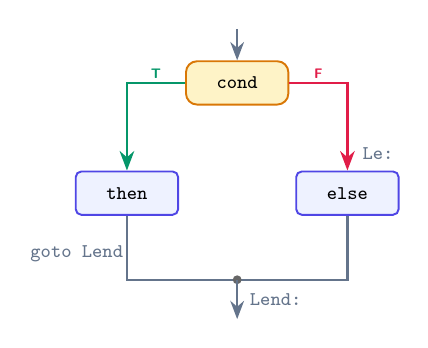
\begin{tikzpicture}[cfg]
          \node[cnd] (c)  at ( 0.0, 0.0) {cond};
          \node[blk] (s1) at (-1.4,-1.4) {then};
          \node[blk] (s2) at ( 1.4,-1.4) {else};
          \coordinate (j) at (0,-2.5);
          \draw[flow] ($(c.north)+(0,0.4)$) -- (c.north);
          \draw[tarr] (c.west) -| node[tf, pos=0.25, above, text=clrT] {T} (s1.north);
          \draw[farr] (c.east) -| node[tf, pos=0.25, above, text=clrF] {F} (s2.north);
          \node[lbl, anchor=west] at ($(s2.north)+( 0.15,0.22)$) {Le:};
          \draw[line] (s1.south) |- node[lbl, left, pos=0.3] {goto Lend} (j);
          \draw[line] (s2.south) |- (j);
          \fill[black!60] (j) circle (1.6pt);
          \draw[flow] (j) -- ++(0,-0.5);
          \node[lbl, anchor=west] at ($(j)+(0.12,-0.25)$) {Lend:};
        \end{tikzpicture}
      \end{center}
      \small The \emph{then} branch needs no label: it is reached by
      falling through. Without \tc{else}, the F exit goes straight to $L_{end}$.
    \end{column}
    \begin{column}{0.48\textwidth}
      \begin{block}{Example}
        \begin{minted}[fontsize=\scriptsize]{c}
if (x > 0) { y = 1; } else { y = 0; }
        \end{minted}
        \vspace{0.3em}
        \begin{minted}[fontsize=\scriptsize]{text}
t1 := x > 0
if_false t1 goto L1
y := 1
goto L2
L1:
y := 0
L2:
        \end{minted}
      \end{block}
    \end{column}
  \end{columns}
\end{frame}

%% ── While ───────────────────────────────────────────────────────────────
\begin{frame}[fragile]{Statements: \tc{while}}
  \begin{columns}[T]
    \begin{column}{0.46\textwidth}
      \textbf{Shape of the generated code:}
      \begin{center}
        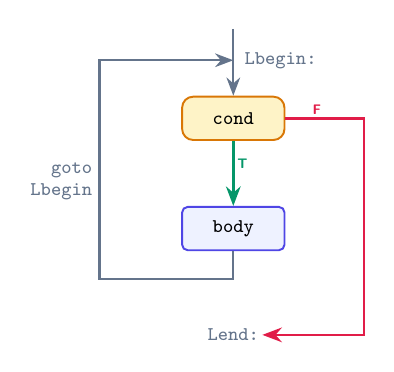
\begin{tikzpicture}[cfg]
          \node[cnd] (c) at (0, 0.0) {cond};
          \node[blk] (b) at (0,-1.4) {body};
          \coordinate (in) at ($(c.north)+(0,0.45)$);
          \node[lbl] (end) at (0,-2.75) {Lend:};
          \draw[flow] ($(in)+(0,0.4)$) -- (c.north);
          \node[lbl, anchor=west] at ($(in)+(0.1,0)$) {Lbegin:};
          \draw[tarr] (c.south) -- node[tf, right, pos=0.35, text=clrT] {T} (b.north);
          \draw[flow] (b.south) -- ++(0,-0.35) -| ($(in)+(-1.7,0)$) -- (in);
          \node[lbl, anchor=east, align=right] at (-1.75,-0.8) {goto\\Lbegin};
          \draw[farr] (c.east) -- node[tf, above, pos=0.4, text=clrF] {F}
                ($(c.east)+(1.0,0)$) |- (end.east);
        \end{tikzpicture}
      \end{center}
      \small The condition is tested \emph{before} each iteration;
      the body falls through and jumps back to the test.
    \end{column}
    \begin{column}{0.48\textwidth}
      \begin{block}{Example}
        \begin{minted}[fontsize=\scriptsize]{c}
while (i < n) { s = s + i; i = i + 1; }
        \end{minted}
        \vspace{0.3em}
        \begin{minted}[fontsize=\scriptsize]{text}
L1:
t1 := i < n
if_false t1 goto L2
t2 := s + i
s  := t2
t3 := i + 1
i  := t3
goto L1
L2:
        \end{minted}
      \end{block}
    \end{column}
  \end{columns}
\end{frame}

%% ── Function calls ──────────────────────────────────────────────────────
\begin{frame}[fragile]{Function Calls}
  \begin{columns}[T]
    \begin{column}{0.50\textwidth}
      \textbf{Idea.} A call \tc{f(e1, ..., en)} becomes:
      \begin{enumerate}
        \item evaluate \textbf{all} arguments first;
        \item push them with \tc{param}, in order;
        \item \tc{call f, n} — $n$ says how many \tc{param}s belong to this call.
      \end{enumerate}
      As an \emph{expression}, the result goes into a fresh temporary:
      \tc{t := call f, n}. As a \emph{statement}, it is discarded.
    \end{column}
    \begin{column}{0.46\textwidth}
      \begin{block}{Nested call}
        \begin{minted}[fontsize=\scriptsize]{c}
x = f(a + 1, g(b));
        \end{minted}
        \vspace{0.2em}
        \begin{minted}[fontsize=\scriptsize]{text}
t1 := a + 1
param b
t2 := call g, 1
param t1
param t2
t3 := call f, 2
x  := t3
        \end{minted}
      \end{block}
    \end{column}
  \end{columns}
\end{frame}

%% ── Functions and return ────────────────────────────────────────────────
\begin{frame}[fragile]{Function Bodies and \tc{return}}
  \begin{columns}[T]
    \begin{column}{0.50\textwidth}
      \textbf{Idea.}
      \begin{itemize}
        \item A function becomes a \textbf{label} with its name,
              followed by the code of its body.
        \item Parameters are ordinary variables inside the body.
        \item \tc{return e} evaluates \tc{e} and emits \tc{return a};
              a plain \tc{return} emits just \tc{return}.
      \end{itemize}
    \end{column}
    \begin{column}{0.46\textwidth}
      \begin{block}{Example}
        \begin{minted}[fontsize=\small]{c}
int sq_sum(int a, int b) {
  return a * a + b * b;
}
        \end{minted}
        \vspace{0.3em}
        \begin{minted}[fontsize=\small]{text}
sq_sum:
a := param0
b := param1
t1 := a * a
t2 := b * b
t3 := t1 + t2
return t3
        \end{minted}
      \end{block}
    \end{column}
  \end{columns}
\end{frame}

%% ── Canonical example ───────────────────────────────────────────────────
\begin{frame}[fragile]{Canonical Example: \tc{while (a[i] < v) \{ i = i + 1; \}}}
  \begin{columns}[T]
    \begin{column}{0.44\textwidth}
      \begin{minted}[fontsize=\small]{c}
while (a[i] < v) {
  i = i + 1;
}
      \end{minted}
      \small Everything we have seen so far, in a single loop:
      \begin{itemize}
        \item the \textbf{loop shape} (\tc{L1}/\tc{L2});
        \item an \textbf{array access} in the condition (offset + load);
        \item the \textbf{condition}: its value, then \tc{if\_false};
        \item an \textbf{assignment} in the body.
      \end{itemize}
    \end{column}
    \begin{column}{0.52\textwidth}
      \begin{block}{Generated TAC}
        \begin{minted}[fontsize=\footnotesize]{text}
L1:                  ; loop test
t1 := i * 8          ; offset of a[i]
t2 := a[t1]          ; a[i]
t3 := t2 < v         ; a[i] < v
if_false t3 goto L2  ; no: leave loop
t4 := i + 1          ; loop body
i  := t4             ; i = i + 1
goto L1              ; back to the test
L2:                  ; after the loop
        \end{minted}
      \end{block}
    \end{column}
  \end{columns}
\end{frame}

%% ── Canonical example as a CFG ──────────────────────────────────────────
\begin{frame}{Canonical Example as a Control-Flow Graph}
  \begin{columns}[T]
    \begin{column}{0.56\textwidth}
      \centering
      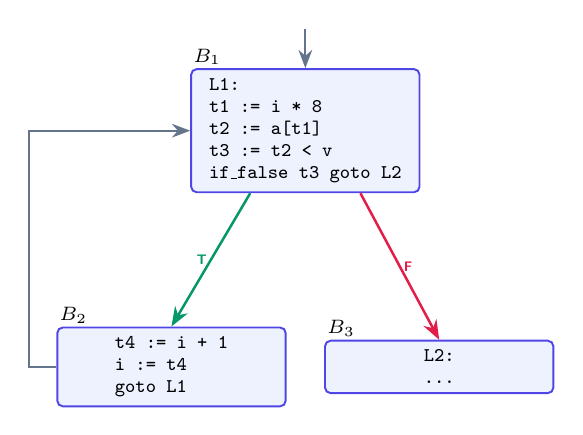
\begin{tikzpicture}[cfg, bb/.style={blk, align=left, minimum width=2.9cm}]
        \node[bb] (B1) at ( 0.0, 0.0) {L1:\\t1 := i * 8\\t2 := a[t1]\\t3 := t2 < v\\if\_false t3 goto L2};
        \node[bb] (B2) at (-1.7,-3.0) {t4 := i + 1\\i := t4\\goto L1};
        \node[bb] (B3) at ( 1.7,-3.0) {L2:\\\ldots};
        \foreach \b/\n in {B1/1, B2/2, B3/3}
          \node[font=\sffamily\scriptsize\bfseries, anchor=south west, inner sep=1pt]
            at (\b.north west) {$B_\n$};
        \draw[flow] ($(B1.north)+(0,0.5)$) -- (B1.north);
        \draw[tarr] ($(B1.south)+(-0.7,0)$) -- node[tf, left, text=clrT] {T} (B2.north);
        \draw[farr] ($(B1.south)+( 0.7,0)$) -- node[tf, right, text=clrF] {F} (B3.north);
        \draw[flow] (B2.west) -- ++(-0.35,0) |- (B1.west);
      \end{tikzpicture}
    \end{column}
    \begin{column}{0.40\textwidth}
      \small
      \textbf{Basic block:} a maximal sequence of instructions that is
      entered only at the first one and left only at the last one.

      \medskip
      \textbf{CFG:} nodes are basic blocks; edges are jumps or fall-throughs.

      \medskip
      Notice the end of $B_1$: \tc{t3} is computed only to be tested
      right away. A single relational jump (\tc{if t2 >= v goto L2})
      would do. Part~III shows how to generate that directly.
    \end{column}
  \end{columns}
\end{frame}

%% ── Arrays ──────────────────────────────────────────────────────────────
\begin{frame}[fragile]{Arrays}
  \begin{columns}[T]
    \begin{column}{0.52\textwidth}
      \textbf{Idea.} Memory is addressed in \emph{bytes}, indices are in
      \emph{elements}. To access \tc{a[i]} we must:
      \begin{enumerate}
        \item evaluate the index \tc{i};
        \item scale it by the element width $w$ (known from the type checker);
        \item load from (or store to) \tc{a} at that offset.
      \end{enumerate}
      Throughout these slides, \tc{int} has width $w = 8$.
    \end{column}
    \begin{column}{0.44\textwidth}
      \begin{block}{Reading: \tc{x = a[i + 1];}}
        \begin{minted}[fontsize=\small]{text}
t1 := i + 1
t2 := t1 * 8
t3 := a[t2]
x  := t3
        \end{minted}
      \end{block}
      \begin{block}{Writing: \tc{a[i] = y + 1;}}
        \begin{minted}[fontsize=\small]{text}
t1 := i * 8
t2 := y + 1
a[t1] := t2
        \end{minted}
      \end{block}
    \end{column}
  \end{columns}
\end{frame}



%% ══════════════════════════════════════════════════════════════════════════
%% ══════════════════════════════════════════════════════════════════════════
\section{Formalization}
%% ══════════════════════════════════════════════════════════════════════════
%% ══════════════════════════════════════════════════════════════════════════

\begin{frame}{Notation}
  \small
  \begin{block}{Translation functions}
    \begin{tabular}{ll}
      $\trExpr{e} \Rightarrow (a,\ I)$     & code $I$ leaves the value of $e$ in address $a$ \\[0.2em]
      $\trCond{c}{L_f} \Rightarrow I$      & code $I$ falls through if $c$ holds, else jumps to $L_f$ \\[0.2em]
      $\trStmt{s} \Rightarrow I$           & code $I$ executes statement $s$ \\[0.2em]
      $\trFun{d} \Rightarrow I$            & code $I$ for function declaration $d$
    \end{tabular}
  \end{block}
  \vspace{0.3em}
  \begin{block}{Conventions}
    \begin{itemize}
      \item $I_1 \cat I_2$ — concatenation of instruction sequences; $[\,\ldots\,]$ — a literal sequence.
      \item ``$t$ fresh'', ``$L$ fresh'' — a new temporary / label, never used before.
      \item $w(T)$ — width in bytes of type $T$ (from the type checker).
    \end{itemize}
  \end{block}
\end{frame}

%% ── trExpr: leaves, binary ops, index ───────────────────────────────────
\begin{frame}{Rules: Expressions}
  \footnotesize
  \[
    \inferrule[Const]{ }{ \trExpr{k} \Rightarrow (k,\ []) }
    \qquad
    \inferrule[Var]{ }{ \trExpr{x} \Rightarrow (x,\ []) }
    \qquad
    \inferrule[Neg]
      { \trExpr{e} \Rightarrow (a,\ I) \\ t\ \text{fresh} }
      { \trExpr{\texttt{-}e} \Rightarrow (t,\ I \cat [\,t := \texttt{-}a\,]) }
  \]
  \vspace{0.6em}
  \[
    \inferrule[BinOp]
      {
        \trExpr{e_1} \Rightarrow (a_1,\ I_1) \\
        \trExpr{e_2} \Rightarrow (a_2,\ I_2) \\
        t\ \text{fresh}
      }
      { \trExpr{e_1 \oplus e_2} \Rightarrow
        \bigl(t,\;I_1 \cat I_2 \cat [\,t := a_1 \oplus a_2\,]\bigr) }
    \qquad \oplus \in \{\tc{+},\tc{-},\tc{*},\tc{/}\}
  \]
  \vspace{0.6em}
  \[
    \inferrule[RelExpr]
      {
        \trExpr{e_1} \Rightarrow (a_1,\ I_1) \\
        \trExpr{e_2} \Rightarrow (a_2,\ I_2) \\
        t\ \text{fresh}
      }
      { \trExpr{e_1 \mathbin{\mathit{rel}} e_2} \Rightarrow
        \bigl(t,\;I_1 \cat I_2 \cat [\,t := a_1 \mathbin{\mathit{rel}} a_2\,]\bigr) }
    \qquad \text{compare with \textsc{JumpRel} (Part III)}
  \]
  \vspace{0.6em}
  \[
    \inferrule[Index]
      {
        \trExpr{e} \Rightarrow (a_i,\ I) \\
        x : T[\,] \\
        t_1,\ t_2\ \text{fresh}
      }
      { \trExpr{x\texttt{[}e\texttt{]}} \Rightarrow
        \bigl(t_2,\;I \cat [\,t_1 := a_i * w(T),\;\; t_2 := x[t_1]\,]\bigr) }
  \]
\end{frame}

%% ── trExpr for booleans ─────────────────────────────────────────────────
\begin{frame}{Rules: Booleans as Values}
  \scriptsize
  \[
    \inferrule[NotExpr]
      { \trExpr{e} \Rightarrow (a,\ I) \\ t,\ L_f,\ L_e\ \text{fresh} }
      {\vcenter{
        \mln{\trExpr{\texttt{!}e} \Rightarrow \bigl(t,\; I
             \cat [\,\texttt{if\_false}\ a\ \texttt{goto}\ L_f,\;\; t := \texttt{false},\;\; \texttt{goto}\ L_e,}
        \mln{\hspace{8.5em} L_f\texttt{:},\;\; t := \texttt{true},\;\; L_e\texttt{:}\,]\bigr)}
      }}
  \]
  \vspace{0.3em}
  \[
    \inferrule[AndExpr]
      {
        \trExpr{e_1} \Rightarrow (a_1,\ I_1) \\
        \trExpr{e_2} \Rightarrow (a_2,\ I_2) \\
        t,\ L_f,\ L_e\ \text{fresh}
      }
      {\vcenter{
        \mln{\trExpr{e_1 \mathbin{\texttt{\&\&}} e_2} \Rightarrow \bigl(t,\; I_1
             \cat [\,\texttt{if\_false}\ a_1\ \texttt{goto}\ L_f\,] \cat I_2
             \cat [\,\texttt{if\_false}\ a_2\ \texttt{goto}\ L_f,}
        \mln{\hspace{8.5em} t := \texttt{true},\;\; \texttt{goto}\ L_e,\;\;
             L_f\texttt{:},\;\; t := \texttt{false},\;\; L_e\texttt{:}\,]\bigr)}
      }}
  \]
  \vspace{0.3em}
  \[
    \inferrule[OrExpr]
      {
        \trExpr{e_1} \Rightarrow (a_1,\ I_1) \\
        \trExpr{e_2} \Rightarrow (a_2,\ I_2) \\
        t,\ L_t,\ L_f,\ L_e\ \text{fresh}
      }
      {\vcenter{
        \mln{\trExpr{e_1 \mathbin{\texttt{||}} e_2} \Rightarrow \bigl(t,\; I_1
             \cat [\,\texttt{if\_false}\ a_1\ \texttt{goto}\ L_f,\;\; \texttt{goto}\ L_t,\;\; L_f\texttt{:}\,]
             \cat I_2 \cat [\,\texttt{if}\ a_2\ \texttt{goto}\ L_t,}
        \mln{\hspace{8.5em} t := \texttt{false},\;\; \texttt{goto}\ L_e,\;\;
             L_t\texttt{:},\;\; t := \texttt{true},\;\; L_e\texttt{:}\,]\bigr)}
      }}
  \]
\end{frame}

%% ── Assignment & sequencing ─────────────────────────────────────────────
\begin{frame}{Rules: Assignment and Blocks}
  \footnotesize
  \[
    \inferrule[Assign]
      { \trExpr{e} \Rightarrow (a,\ I) }
      { \trStmt{x\ \texttt{=}\ e} \Rightarrow I \cat [\,x := a\,] }
    \qquad
    \inferrule[Decl]
      { \trExpr{e} \Rightarrow (a,\ I) }
      { \trStmt{T\ x\ \texttt{=}\ e} \Rightarrow I \cat [\,x := a\,] }
  \]
  \vspace{0.6em}
  \[
    \inferrule[Store]
      {
        \trExpr{e_1} \Rightarrow (a_i,\ I_1) \\
        \trExpr{e_2} \Rightarrow (a,\ I_2) \\
        x : T[\,] \\
        t\ \text{fresh}
      }
      { \trStmt{x\texttt{[}e_1\texttt{]}\ \texttt{=}\ e_2} \Rightarrow
        I_1 \cat [\,t := a_i * w(T)\,] \cat I_2 \cat [\,x[t] := a\,] }
  \]
  \vspace{0.6em}
  \[
    \inferrule[Block]
      { \trStmt{s_i} \Rightarrow I_i \quad (1 \le i \le n) }
      { \trStmt{\texttt{\{}\,s_1 \ldots s_n\,\texttt{\}}} \Rightarrow I_1 \cat \cdots \cat I_n }
  \]
\end{frame}

%% ── Conditions and if ───────────────────────────────────────────────────
\begin{frame}{Rules: Conditions and \tc{if}}
  \footnotesize
  \[
    \inferrule[Cond]
      { \trExpr{c} \Rightarrow (a,\ I) }
      { \trCond{c}{L_f} \Rightarrow I \cat [\,\texttt{if\_false}\ a\ \texttt{goto}\ L_f\,] }
    \quad \text{\scriptsize(a single rule: \texttt{\&\&}, \texttt{||}, \texttt{!} are handled by $\mathit{trExpr}$)}
  \]
  \vspace{0.8em}
  \[
    \inferrule[IfElse]
      {
        L_e,\ L_{\mathit{end}}\ \text{fresh} \\
        \trCond{c}{L_e} \Rightarrow I_c \\
        \trStmt{s_1} \Rightarrow I_1 \\
        \trStmt{s_2} \Rightarrow I_2
      }
      {\vcenter{
        \mln{\trStmt{\texttt{if}\,(c)\;s_1\;\texttt{else}\;s_2} \Rightarrow
             I_c \cat I_1 \cat [\,\texttt{goto}\ L_{\mathit{end}},\;\; L_e\texttt{:}\,]}
        \mln{\hspace{10em}\cat I_2 \cat [\,L_{\mathit{end}}\texttt{:}\,]}
      }}
  \]
  \vspace{0.8em}
  \[
    \inferrule[If]
      {
        L_{\mathit{end}}\ \text{fresh} \\
        \trCond{c}{L_{\mathit{end}}} \Rightarrow I_c \\
        \trStmt{s} \Rightarrow I
      }
      { \trStmt{\texttt{if}\,(c)\;s} \Rightarrow
        I_c \cat I \cat [\,L_{\mathit{end}}\texttt{:}\,] }
  \]
\end{frame}

%% ── Loops ───────────────────────────────────────────────────────────────
\begin{frame}{Rules: \tc{while}}
  \footnotesize
  \[
    \inferrule[While]
      {
        L_b,\ L_{\mathit{end}}\ \text{fresh} \\
        \trCond{c}{L_{\mathit{end}}} \Rightarrow I_c \\
        \trStmt{s} \Rightarrow I
      }
      { \trStmt{\texttt{while}\,(c)\;s} \Rightarrow
        [\,L_b\texttt{:}\,] \cat I_c \cat I \cat [\,\texttt{goto}\ L_b,\;\; L_{\mathit{end}}\texttt{:}\,] }
  \]
  \medskip
  \normalsize
  $L_b$ is the target of the back-edge; $L_{\mathit{end}}$ is the only exit
  handed to $\mathit{trCond}$. The body is reached by falling through.
\end{frame}

%% ── Calls and return ────────────────────────────────────────────────────
\begin{frame}{Rules: Calls, \tc{return} and Functions}
  \footnotesize
  \[
    \inferrule[CallExpr]
      {
        \trExpr{e_i} \Rightarrow (a_i,\ I_i) \quad (1 \le i \le n) \\
        t\ \text{fresh}
      }
      { \trExpr{f(e_1,\ldots,e_n)} \Rightarrow
        \bigl(t,\; I_1 \cat \cdots \cat I_n \cat
        [\,\texttt{param}\ a_1, \ldots, \texttt{param}\ a_n,\;\; t := \texttt{call}\ f, n\,]\bigr) }
  \]
  \vspace{0.5em}
  \[
    \inferrule[CallStmt]
      { \trExpr{e_i} \Rightarrow (a_i,\ I_i) \quad (1 \le i \le n) }
      { \trStmt{f(e_1,\ldots,e_n)} \Rightarrow
        I_1 \cat \cdots \cat I_n \cat
        [\,\texttt{param}\ a_1, \ldots, \texttt{param}\ a_n,\;\; \texttt{call}\ f, n\,] }
  \]
  \vspace{0.5em}
  \[
    \inferrule[Return]
      { \trExpr{e} \Rightarrow (a,\ I) }
      { \trStmt{\texttt{return}\ e} \Rightarrow I \cat [\,\texttt{return}\ a\,] }
    \qquad
    \inferrule[ReturnVoid]{ }{ \trStmt{\texttt{return}} \Rightarrow [\,\texttt{return}\,] }
  \]
  \vspace{0.5em}
  \[
    \inferrule[Fun]
      { \trStmt{s} \Rightarrow I }
      { \trFun{T\ f(p_1,\ldots,p_n)\ s} \Rightarrow [\,f\texttt{:}\,] \cat I }
  \]
\end{frame}

%% ── Derivation of the canonical example ─────────────────────────────────
\begin{frame}[fragile]{Putting It Together: Deriving the Canonical Example}
  \begin{columns}[T]
    \begin{column}{0.56\textwidth}
      \scriptsize
      \textsc{While} picks $L_b = \tc{L1}$, $L_{\mathit{end}} = \tc{L2}$:
      \[
        \begin{array}{l}
        [\,\tc{L1:}\,] \cat \underbrace{\trCond{\tc{a[i] < v}}{\tc{L2}}}_{I_c} \\[1.2em]
        \quad \cat \underbrace{\trStmt{\tc{i = i + 1}}}_{I}
        \cat [\,\tc{goto L1},\; \tc{L2:}\,]
        \end{array}
      \]
      \begin{itemize}
        \item $I_c$: \textsc{Cond} over \textsc{RelExpr}(\textsc{Index}, \textsc{Var})
          \begin{itemize}
            \item \textsc{Index}: \tc{t1 := i * 8;\ t2 := a[t1]}, address \tc{t2}
            \item \textsc{Var}: address \tc{v}, no code
            \item \textsc{RelExpr}: \tc{t3 := t2 < v}
            \item \textsc{Cond}: \tc{if\_false t3 goto L2}
          \end{itemize}
        \item $I$: \textsc{Assign} over \textsc{BinOp}(\textsc{Var}, \textsc{Const})
              $\Rightarrow$ \tc{t4 := i + 1;\ i := t4}
      \end{itemize}
    \end{column}
    \begin{column}{0.40\textwidth}
      \begin{block}{Result}
        \begin{minted}[fontsize=\small]{text}
L1:                  ; While
t1 := i * 8          ; Index
t2 := a[t1]          ; Index
t3 := t2 < v         ; RelExpr
if_false t3 goto L2  ; Cond
t4 := i + 1          ; BinOp
i  := t4             ; Assign
goto L1              ; While
L2:                  ; While
        \end{minted}
      \end{block}
    \end{column}
  \end{columns}
\end{frame}

%% ══════════════════════════════════════════════════════════════════════════
%% ══════════════════════════════════════════════════════════════════════════
\section{Refinement: Jumping Code}
%% ══════════════════════════════════════════════════════════════════════════
%% ══════════════════════════════════════════════════════════════════════════

%% ── Motivation ──────────────────────────────────────────────────────────
\begin{frame}[fragile]{Why Refine?}
  \begin{columns}[T]
    \begin{column}{0.40\textwidth}
      \begin{block}{Value, then test (Part II)}
        \begin{minted}[fontsize=\scriptsize]{text}
t1 := x > 0
if_false t1 goto L1
t2 := y < 10
if_false t2 goto L1
t3 := true
goto L2
L1:
t3 := false
L2:
if_false t3 goto Lelse
<then>
        \end{minted}
      \end{block}
    \end{column}
    \begin{column}{0.30\textwidth}
      \begin{block}{Jumping code}
        \begin{minted}[fontsize=\scriptsize]{text}
if x > 0 goto L1
goto Lelse
L1:
if y < 10 goto Lthen
goto Lelse
Lthen:
<then>
        \end{minted}
      \end{block}
    \end{column}
    \begin{column}{0.26\textwidth}
      \small
      Both translate \tc{if (x > 0 \&\& y < 10)}.

      \medskip
      On the left, the boolean \tc{t3} is built only to be tested once.
      \emph{Jumping code} turns the condition directly into control flow:
      no temporaries, fewer instructions.
    \end{column}
  \end{columns}

  \medskip
  \small
  \textbf{Price:} a second translation function,
  $\trJump{c}{L_t}{L_f}$, with one rule per logical operator.
\end{frame}

\begin{frame}[fragile]{Jumping Code: Two Exits}
  \begin{columns}[T]
    \begin{column}{0.52\textwidth}
In \textbf{jumping code}, a condition is
      a box with one entry and \textbf{two exits}.
      \begin{center}
        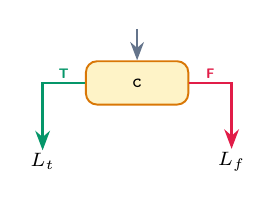
\begin{tikzpicture}[cfg]
          \node[cnd] (c) at (0,0) {c};
          \node[exit] (lt) at (-1.2,-1.0) {$L_t$};
          \node[exit] (lf) at ( 1.2,-1.0) {$L_f$};
          \draw[flow] ($(c.north)+(0,0.4)$) -- (c.north);
          \draw[tarr] (c.west) -| node[tf, pos=0.25, above, text=clrT] {T} (lt.north);
          \draw[farr] (c.east) -| node[tf, pos=0.25, above, text=clrF] {F} (lf.north);
        \end{tikzpicture}
      \end{center}
      The enclosing statement decides what $L_t$ and $L_f$ are.
    \end{column}
    \begin{column}{0.44\textwidth}
      \begin{block}{Relational: \tc{x < y}}
        \begin{minted}[fontsize=\scriptsize]{text}
if x < y goto Lt
goto Lf
        \end{minted}
      \end{block}
      \begin{block}{Boolean variable: \tc{flag}}
        \begin{minted}[fontsize=\scriptsize]{text}
if flag goto Lt
goto Lf
        \end{minted}
      \end{block}
      \begin{block}{Literals}
        \begin{minted}[fontsize=\scriptsize]{text}
true   ==>  goto Lt
false  ==>  goto Lf
        \end{minted}
      \end{block}
    \end{column}
  \end{columns}
\end{frame}

%% ── Short-circuit: diagrams ─────────────────────────────────────────────
\begin{frame}{Conditions: \tc{\&\&}, \tc{||} and \tc{!} by Rewiring Exits}
  \textbf{Idea.} The logical operators do not compute anything:
  they only \emph{rewire} the T/F exits of their operands.
  Short-circuit evaluation comes for free.

  \medskip
  \begin{columns}[T]
    \begin{column}{0.32\textwidth}
      \centering
      \textbf{\tc{c1 \&\& c2}}\\[0.4em]
      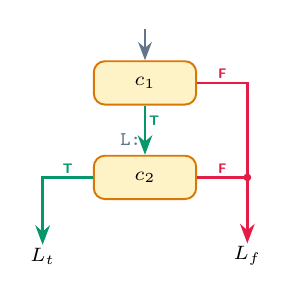
\begin{tikzpicture}[cfg]
        \node[cnd]  (c1) at (0, 0)    {$c_1$};
        \node[cnd]  (c2) at (0,-1.2)  {$c_2$};
        \node[exit] (lt) at (-1.3,-2.2) {$L_t$};
        \node[exit] (lf) at ( 1.3,-2.2) {$L_f$};
        \draw[flow] ($(c1.north)+(0,0.4)$) -- (c1.north);
        \draw[tarr] (c1.south) -- node[tf, right, pos=0.3, text=clrT] {T}
                                  node[lbl, left, pos=0.7] {L:} (c2.north);
        \draw[farr] (c1.east) -| node[tf, pos=0.25, above, text=clrF] {F} (lf.north);
        \draw[tarr] (c2.west) -| node[tf, pos=0.25, above, text=clrT] {T} (lt.north);
        \draw[line, draw=clrF, line width=0.9pt] (c2.east) --
              node[tf, above, text=clrF] {F} (c2.east -| lf.north);
        \fill[clrF] (c2.east -| lf.north) circle (1.4pt);
      \end{tikzpicture}\\[0.4em]
      \raggedright\scriptsize $c_1$ false $\Rightarrow$ straight to $L_f$;
      $c_2$ is never evaluated.
    \end{column}
    \begin{column}{0.32\textwidth}
      \centering
      \textbf{\tc{c1 || c2}}\\[0.4em]
      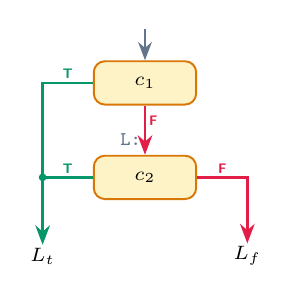
\begin{tikzpicture}[cfg]
        \node[cnd]  (c1) at (0, 0)    {$c_1$};
        \node[cnd]  (c2) at (0,-1.2)  {$c_2$};
        \node[exit] (lt) at (-1.3,-2.2) {$L_t$};
        \node[exit] (lf) at ( 1.3,-2.2) {$L_f$};
        \draw[flow] ($(c1.north)+(0,0.4)$) -- (c1.north);
        \draw[tarr] (c1.west) -| node[tf, pos=0.25, above, text=clrT] {T} (lt.north);
        \draw[farr] (c1.south) -- node[tf, right, pos=0.3, text=clrF] {F}
                                  node[lbl, left, pos=0.7] {L:} (c2.north);
        \draw[line, draw=clrT, line width=0.9pt] (c2.west) --
              node[tf, above, text=clrT] {T} (c2.west -| lt.north);
        \fill[clrT] (c2.west -| lt.north) circle (1.4pt);
        \draw[farr] (c2.east) -| node[tf, pos=0.25, above, text=clrF] {F} (lf.north);
      \end{tikzpicture}\\[0.4em]
      \raggedright\scriptsize $c_1$ true $\Rightarrow$ straight to $L_t$;
      $c_2$ is never evaluated.
    \end{column}
    \begin{column}{0.32\textwidth}
      \centering
      \textbf{\tc{!c}}\\[0.4em]
      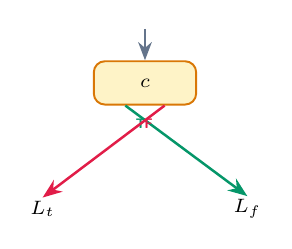
\begin{tikzpicture}[cfg]
        \node[cnd]  (c)  at (0,-0.6)  {$c$};
        \node[exit] (lt) at (-1.3,-2.2) {$L_t$};
        \node[exit] (lf) at ( 1.3,-2.2) {$L_f$};
        \draw[flow] ($(c.north)+(0,0.4)$) -- (c.north);
        \draw[tarr] ($(c.south)+(-0.25,0)$) --
              node[tf, left, pos=0.2, text=clrT] {T} (lf.north);
        \draw[farr] ($(c.south)+(0.25,0)$) --
              node[tf, right, pos=0.2, text=clrF] {F} (lt.north);
      \end{tikzpicture}\\[0.4em]
      \raggedright\scriptsize The exits of $c$ \textbf{cross}: its T exit
      becomes $L_f$ and vice versa. No code at all.
    \end{column}
  \end{columns}
\end{frame}

%% ── Short-circuit: generated TAC ────────────────────────────────────────
\begin{frame}[fragile]{Conditions: \tc{\&\&}, \tc{||} and \tc{!} in TAC}
  The intermediate label \tc{L} in the diagrams becomes a fresh label (\tc{L1}):

  \medskip
  \begin{columns}[T]
    \begin{column}{0.32\textwidth}
      \begin{block}{\tc{x > 0 \&\& y < 10}}
        \begin{minted}[fontsize=\scriptsize]{text}
if x > 0 goto L1
goto Lf
L1:
if y < 10 goto Lt
goto Lf
        \end{minted}
      \end{block}
      \scriptsize If the left side is false, go straight to $L_f$.
    \end{column}
    \begin{column}{0.32\textwidth}
      \begin{block}{\tc{found || n < 10}}
        \begin{minted}[fontsize=\scriptsize]{text}
if found goto Lt
goto L1
L1:
if n < 10 goto Lt
goto Lf
        \end{minted}
      \end{block}
      \scriptsize If the left side is true, go straight to $L_t$.
    \end{column}
    \begin{column}{0.32\textwidth}
      \begin{block}{\tc{!(x < y)}}
        \begin{minted}[fontsize=\scriptsize]{text}
if x < y goto Lf
goto Lt
        \end{minted}
      \end{block}
      \scriptsize Negation just \textbf{swaps} $L_t$ and $L_f$ — no code at all.
    \end{column}
  \end{columns}
\end{frame}

%% ── trCond: base cases and relational ───────────────────────────────────
\begin{frame}{Rules: Jumping Code — Base Cases}
  \footnotesize
  \[
    \inferrule[JumpTrue]{ }{ \trJump{\texttt{true}}{L_t}{L_f} \Rightarrow [\,\texttt{goto}\ L_t\,] }
    \qquad
    \inferrule[JumpFalse]{ }{ \trJump{\texttt{false}}{L_t}{L_f} \Rightarrow [\,\texttt{goto}\ L_f\,] }
  \]
  \vspace{0.6em}
  \[
    \inferrule[JumpRel]
      {
        \trExpr{e_1} \Rightarrow (a_1,\ I_1) \\
        \trExpr{e_2} \Rightarrow (a_2,\ I_2)
      }
      { \trJump{e_1 \mathbin{\mathit{rel}} e_2}{L_t}{L_f} \Rightarrow
        I_1 \cat I_2 \cat [\,\texttt{if}\ a_1 \mathbin{\mathit{rel}} a_2\ \texttt{goto}\ L_t,\;\; \texttt{goto}\ L_f\,] }
  \]
  \centerline{$\mathit{rel} \in \{\tc{<},\tc{<=},\tc{>},\tc{>=},\tc{==},\tc{!=}\}$}
  \vspace{0.6em}
  \[
    \inferrule[JumpExpr]
      { \trExpr{e} \Rightarrow (a,\ I) }
      { \trJump{e}{L_t}{L_f} \Rightarrow
        I \cat [\,\texttt{if}\ a\ \texttt{goto}\ L_t,\;\; \texttt{goto}\ L_f\,] }
    \quad \text{\scriptsize(any other boolean $e$, e.g.\ a variable or a call)}
  \]
\end{frame}

%% ── trCond: logical operators ───────────────────────────────────────────
\begin{frame}{Rules: Jumping Code — Logical Operators}
  \footnotesize
  \[
    \inferrule[JumpAnd]
      {
        L\ \text{fresh} \\
        \trJump{c_1}{L}{L_f} \Rightarrow I_1 \\
        \trJump{c_2}{L_t}{L_f} \Rightarrow I_2
      }
      { \trJump{c_1 \mathbin{\texttt{\&\&}} c_2}{L_t}{L_f} \Rightarrow
        I_1 \cat [\,L\texttt{:}\,] \cat I_2 }
  \]
  \vspace{0.6em}
  \[
    \inferrule[JumpOr]
      {
        L\ \text{fresh} \\
        \trJump{c_1}{L_t}{L} \Rightarrow I_1 \\
        \trJump{c_2}{L_t}{L_f} \Rightarrow I_2
      }
      { \trJump{c_1 \mathbin{\texttt{||}} c_2}{L_t}{L_f} \Rightarrow
        I_1 \cat [\,L\texttt{:}\,] \cat I_2 }
  \]
  \vspace{0.6em}
  \[
    \inferrule[JumpNot]
      { \trJump{c}{L_f}{L_t} \Rightarrow I }
      { \trJump{\texttt{!}c}{L_t}{L_f} \Rightarrow I }
  \]
  \medskip
  \normalsize
  Note how \textsc{JumpAnd} / \textsc{JumpOr} only differ in \emph{which exit}
  of $c_1$ is redirected to $L$, and \textsc{JumpNot} swaps the exits.
\end{frame}

%% ── Statements with jumping code ────────────────────────────────────────
\begin{frame}{Rules: Statements with Jumping Code}
  \footnotesize
  \[
    \inferrule[JumpIfElse]
      {
        L_t,\ L_e,\ L_{\mathit{end}}\ \text{fresh} \\
        \trJump{c}{L_t}{L_e} \Rightarrow I_c \\
        \trStmt{s_1} \Rightarrow I_1 \\
        \trStmt{s_2} \Rightarrow I_2
      }
      {\vcenter{
        \mln{\trStmt{\texttt{if}\,(c)\;s_1\;\texttt{else}\;s_2} \Rightarrow
             I_c \cat [\,L_t\texttt{:}\,] \cat I_1 \cat [\,\texttt{goto}\ L_{\mathit{end}}\,]}
        \mln{\hspace{10em}\cat [\,L_e\texttt{:}\,] \cat I_2 \cat [\,L_{\mathit{end}}\texttt{:}\,]}
      }}
  \]
  \vspace{1em}
  \[
    \inferrule[JumpWhile]
      {
        L_b,\ L_{\mathit{body}},\ L_{\mathit{end}}\ \text{fresh} \\
        \trJump{c}{L_{\mathit{body}}}{L_{\mathit{end}}} \Rightarrow I_c \\
        \trStmt{s} \Rightarrow I
      }
      {\vcenter{
        \mln{\trStmt{\texttt{while}\,(c)\;s} \Rightarrow
             [\,L_b\texttt{:}\,] \cat I_c \cat [\,L_{\mathit{body}}\texttt{:}\,]}
        \mln{\hspace{8em}\cat I \cat [\,\texttt{goto}\ L_b,\;\; L_{\mathit{end}}\texttt{:}\,]}
      }}
  \]
  \medskip
  \normalsize
  Both exits are now explicit jumps, so the \emph{then} branch and the loop
  body need a label ($L_t$, $L_{\mathit{body}}$) again.
\end{frame}

\end{document}
